% =====================================================================
\section{Experiments}
\label{sec:results}
% =====================================================================

The central result is at the item level (\cref{sec:itemlevel}); we build to
it---setup, the average effect, a sensitivity check---then analyse it directly.

\subsection{Setup}
\label{sec:setup}
Our primary model is \textbf{Qwen3.5-9B} fine-tuned with
LoRA~\cite{lora_2022} (rank \num{16}, $\alpha=\num{16}$, all linear layers including
the vision tower, bfloat16, max image edge \num{512}\,px) on the seen/unseen
training split. We train it at the \emph{minimum-sufficient} input---a marked
satellite tile plus the single \emph{forward} street view (\textsf{satfwd}), two
images per sample---so that every comparison sits on the same one-street-view
regime. Fine-tuning on the task distribution is deliberate: a failure to use both
views then cannot be blamed on poor task alignment.
For the mismatch tasks, which structurally require comparing the full street-view
set against the satellite tile, evaluation feeds all four street views even to this
adapter, because the task design forces it.

We evaluate under the three image-ablation conditions of \cref{sec:protocol}:
\textsf{sat} (marked tile), \textsf{sv} (forward street view), and \textsf{full}
(both). In this configuration \textsf{full} means \emph{two} images---one satellite,
one street view; we report the four-street-view training regime separately in
\cref{sec:supp}. The quantity of interest is \emph{fusion synergy}
$=\textsf{full}-\max(\textsf{sat},\textsf{sv})$, the gain of both views over the
better single one. To check that the finding is not model-specific we also evaluate
four off-the-shelf, overhead-only remote-sensing VLMs zero-shot (\cref{tab:models};
\cref{sec:zeroshot}) and a panel of raw open VLMs under the same conditions
(\cref{sec:replication}); all run through one harness on a single \SI{96}{GB} GPU.

\subsection{The second view adds little over the better single view}
\label{sec:main}

Does adding the second view improve average accuracy? \Cref{tab:fusion-main}
reports the trained model per urban task under the three conditions. \textsf{full}
tracks the \emph{better single view} closely: per-task fusion synergy ranges from
$-\num{2.4}$ (\textsf{amenity\_richness}) to $+\num{2.9}$ (\textsf{transit\_density})
and averages $+\num{0.5}$ points across the seven tasks; two tasks have
\emph{negative} synergy, and street view alone already matches or exceeds
\textsf{full} on \textsf{road\_type}. Pooled, synergy is $+\num{1.1}$ points
(\num{95}\% CI $[-\num{0.2},+\num{2.4}]$, including zero). The model is plainly
reading the imagery---each single view lands far above the \num{25.2}\% chance rate
of always answering `A', the lowest being \textsf{transit\_density} at \num{46.1}\%
on the weaker view---so the issue is not that the pixels go unused but that the
second view's pixels carry about a single view's worth of usable information.

\begin{table}[t]
  \centering
  \caption{Trained Qwen3.5-9B (\textsf{satfwd}) on the held-out benchmark, per urban
  task and input condition (accuracy, \%). \textbf{Syn.}
  $=\textsf{full}-\max(\textsf{sat},\textsf{sv})$ is fusion synergy. Synergy is small
  on every task and \textsf{full} stays close to the better single view; each single
  view alone is already well above the \num{25.2}\% chance rate.}
  \label{tab:fusion-main}
  \setlength{\tabcolsep}{6pt}
  \begin{tabular}{@{}lrcccr@{}}
    \toprule
    Task & $n$ & sat & sv & full & Syn. \\
    \midrule
    land\_use         & 421 & 72.4 & 71.7 & 72.9 & $+0.5$ \\
    building\_height  & 190 & 60.0 & 62.6 & 63.7 & $+1.1$ \\
    urban\_density    & 421 & 69.6 & 59.1 & 70.1 & $+0.5$ \\
    road\_type        & 421 & 72.7 & 76.0 & 74.6 & $-1.4$ \\
    junction\_type    & 334 & 71.6 & 66.5 & 74.0 & $+2.4$ \\
    amenity\_richness & 421 & 55.3 & 47.7 & 53.0 & $-2.4$ \\
    transit\_density  & 421 & 46.3 & 46.1 & 49.2 & $+2.9$ \\
    \midrule
    \textbf{Mean}     & --- & 64.0 & 61.4 & 65.3 & $\mathbf{+0.5}$ \\
    \bottomrule
  \end{tabular}
\end{table}

A synergy near zero is only meaningful if the instrument can detect fusion when
fusion is present.

\subsection{The instrument is not blind to fusion (sensitivity check)}
\label{sec:control}

The five cross-view tasks check that the same ablation registers fusion where fusion
is genuinely present. They are constructed so the answer lives in the correspondence
between the two views---and, for the mismatch tasks, so the candidate street-view set
that matches the tile is literally one of the options---so removing a view is, by
design, costly. It is: with both views the model reaches \num{87}--\num{98}\% on the
mismatch tasks (\cref{tab:control}), far above either single view. The instrument that
records a half-point change on the urban tasks is plainly not insensitive, so the
urban null is a real absence of synergy. We do \emph{not} read these magnitudes as a
fusion ``score'': the comparison is not image-count-matched (the mismatch tasks feed
the full street-view set), and a large drop when an answer-bearing view is withheld is
expected by design. The image-count-matched question---does a second \emph{modality}
help added to the first?---is the urban one (\cref{sec:main,sec:itemlevel}), where
\textsf{full} adds exactly one street view to one satellite tile.

\begin{table}[t]
  \centering
  \caption{Sensitivity check: the same trained model on the cross-view tasks, whose
  answers depend on the relationship between the views (the mismatch tasks include the
  matching view among the options). The large \textsf{full}-vs-single gap confirms the
  ablation is not blind to fusion; we treat it as a check on the instrument, not as an
  image-count-matched measurement.}
  \label{tab:control}
  \setlength{\tabcolsep}{6pt}
  \begin{tabular}{@{}lcccr@{}}
    \toprule
    Cross-view task & sat & sv & full & Syn. \\
    \midrule
    camera\_direction      & 23.0 & --   & 42.0 & $+19.0$ \\
    mismatch\_binary\_easy & 47.0 & 53.4 & 97.6 & $+44.2$ \\
    mismatch\_binary\_hard & 48.0 & 44.2 & 92.4 & $+44.4$ \\
    mismatch\_mcq\_easy    & 26.1 & 23.8 & 96.9 & $+70.8$ \\
    mismatch\_mcq\_hard    & 22.6 & 24.9 & 87.2 & $+62.2$ \\
    \bottomrule
  \end{tabular}
\end{table}

\subsection{Item-level: the second view interferes more than it helps}
\label{sec:itemlevel}

A small positive average could still hide genuine fusion on a subset of items. We
join the three conditions' predictions at the item level---every question carries a
stable identifier shared across conditions---and analyse the \num{2629} fully paired
urban items directly (\cref{fig:itemlevel}).

\begin{figure}[t]
  \centering
  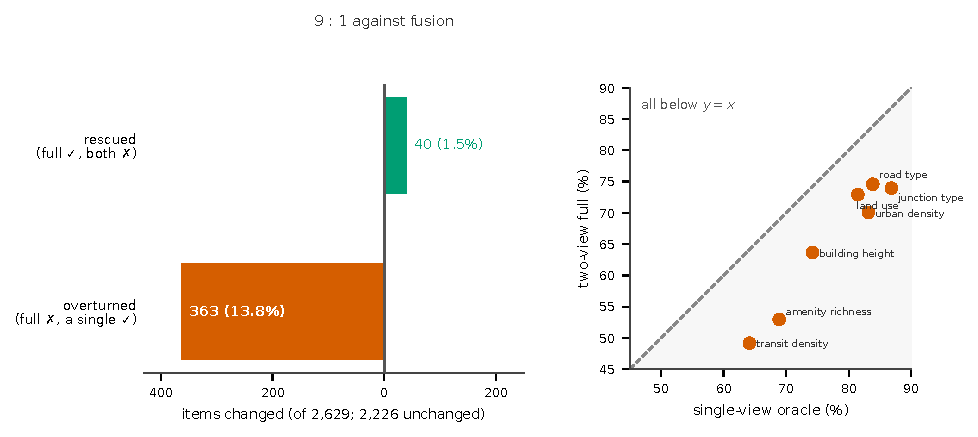
\includegraphics[width=\linewidth]{figures_new/fig_item_combined.pdf}
  \caption{\textbf{Left:} of the \num{2629} urban items, the second view changes
  \num{403}---it rescues \num{40} (both single views missed) and overturns \num{363}
  (a single view had it right), a \num{9}:1 imbalance against fusion. \textbf{Right:}
  per task, two-view accuracy ($y$) versus an oracle keeping the better single view
  per item ($x$; an upper bound, not an achievable system). Every task lies below
  $y=x$. Trained Qwen3.5-9B (\textsf{satfwd}).}
  \label{fig:itemlevel}
\end{figure}

\paragraph{The second view overturns far more correct answers than it rescues.}
Genuine fusion is rare: \textsf{full} is correct while \emph{both} single views are
wrong on only \num{40} items (\num{1.5}\%). Interference is common: \textsf{full} is
wrong while at least one single view was right on \num{363} items (\num{13.8}\%). The
second view therefore overturns a correct answer about nine times as often as it
rescues a wrong one. Equivalently---and this is the \emph{same} statistic stated as
an upper bound---an \emph{oracle} that keeps the better of the two single-view
answers per item (a router, not a fusion model, and not an achievable system, since
selecting the right view uses the gold label) beats \textsf{full} by \num{12.3}
points (\num{77.5} vs.\ \num{65.2}; paired bootstrap \num{95}\% CI
$[\num{10.9},\num{13.7}]$; McNemar $p<\num{e-60}$). The two-view model is beaten by a
single-view router on every one of the seven tasks (\cref{fig:itemlevel}). Against the
street-only view, \textsf{full} is significantly \emph{worse} than parity
($p<\num{e-4}$); against the satellite-only view the win/loss split is not
significant (\num{174} vs.\ \num{145}, $p=\num{0.12}$). When the two views disagree,
the combined input does not reliably preserve the correct answer.

\paragraph{Stronger reasoning does not remove it.}
Perhaps the second view is complementary and the model merely fails to combine
it---in which case stronger inference-time reasoning should surface the signal. It
does not: across plain decoding, a \num{16}k-token
explicit-reasoning budget, and a four-turn observe--reason--self-check--commit
protocol, mean accuracy rises modestly while fusion synergy stays \emph{negative} and
street-view-alone remains the single strongest condition (evaluated on an
AWQ-quantised Qwen3.5-9B so the long-context runs fit one GPU; this probe is an
internal trend check, not numerically comparable to the headline, and the claim rests
only on the sign of synergy, which quantisation does not flip). More deliberation
raises single-view accuracy without raising synergy.

\paragraph{The average gain, precisely.}
The pooled synergy of $+\num{1.1}$ points (CI $[-\num{0.2},+\num{2.4}]$) is
statistically equivalent to zero under a $\pm\num{3}$-point
TOST~\cite{lakens2018tost}. The \emph{harm}, by contrast, is significant: the
single-view oracle's lead has an interval well clear of zero. Whether a near-zero
gain at that interference cost warrants serving a second imagery modality is the
practical question we take up in \cref{sec:discussion}.

\subsection{The finding holds zero-shot across off-the-shelf RS-VLMs}
\label{sec:zeroshot}

To rule out that the redundancy is an artefact of our particular model, we evaluate
four off-the-shelf remote-sensing VLMs (GeoChat, SkySenseGPT, LHRS-Bot-Nova,
EarthDial) zero-shot on the satellite-only half of the urban benchmark. None was
trained on our task, our four-way format, or our marker overlay; they span CLIP- and
SigLIP-based encoders, three LLM families, and single-crop versus tiled
preprocessing. A fine-tuned model
should of course beat zero-shot baselines; the comparison bears not on synergy but on
the single-overhead-view floor. The best zero-shot model (EarthDial, \num{37.8}\%) trails our trained model's
satellite-only accuracy (\num{64.0}\%) by \num{26} points. As unweighted means over
the same seven urban tasks, GeoChat scores \num{21.0}\%, SkySenseGPT \num{27.2}\%,
LHRS-Bot-Nova \num{29.5}\%, and EarthDial \num{37.8}\%; the latter two are trained on
OSM-derived text and are an upper bound on visual skill (\cref{sec:robustness}).

\subsection{The regime split reproduces across families and scales}
\label{sec:replication}

Is the dissociation specific to our fine-tuned model? The same ablation on
raw, zero-shot open VLMs---Qwen3.5-4B/9B,
Qwen2.5-VL-7B, and Gemma-4-12B---preserves the \emph{shape} of the result.
The raw models are weaker overall (urban \textsf{full} accuracy clusters near
\num{50}\% across all four, versus \num{65}\% for our trained model), but the
pattern is the same: a small urban fusion gain and a large cross-view fusion gain.
On the raw Qwen3.5-9B, for instance, urban synergy is essentially zero (and slightly
negative on \textsf{land\_use} and \textsf{junction\_type}), while
\textsf{mismatch\_mcq\_easy} jumps from \num{25}\% with the satellite alone to
\num{66}\% with both views. We evaluate the raw panel under each model's native
street-view scheme, so it speaks only to whether the qualitative regime split recurs,
not to a like-for-like view-count comparison. If anything this grants the panel more
street-view evidence to fuse, making the near-zero urban synergy it still shows a
conservative reading. The regime split is thus a property of current
VLMs and current paired-view tasks, not a fine-tuning artefact.

\subsection{Inference-time view pruning}
\label{sec:pruning}

If a single street view carries the urban signal, pruning the others at inference
should cost little. We measure this on a stronger raw model (Qwen3.6-27B) with a
single metric throughout: among the questions the model already answers correctly
with all street views, what fraction \emph{survive}---stay correct---when the
street-view set is cut to $k$ images (\cref{fig:prune}). At $k{=}\num{1}$, keeping
the forward view retains \num{89}\% of those correct answers, essentially matching
the attention-selected best view (\num{90}\%) and edging out a random view
(\num{85}\%) or the worst (\num{83}\%); one well-chosen street view is almost as good
as four. Cutting to $k{=}\num{0}$ (no street view, satellite only) still retains
\num{67}\%---reflecting residual text and label signal---so no \emph{specific} single
view is essential, and the gap between informed and random selection is small.

\begin{figure}[t]
  \centering
  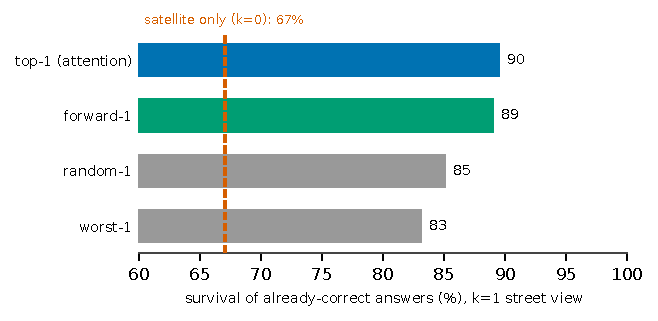
\includegraphics[width=0.74\linewidth]{figures_new/fig_prune.pdf}
  \caption{Survival of already-correct answers as the street-view set is pruned
  (Qwen3.6-27B). Every bar is the same quantity---the fraction of questions correct
  with all views that remain correct after pruning. Keeping one street view
  ($k{=}\num{1}$, any rule) retains \num{83}--\num{90}\%; keeping none
  ($k{=}\num{0}$, satellite only) retains \num{67}\%. This is retention over
  already-correct items, never an accuracy.}
  \label{fig:prune}
\end{figure}

\subsection{What do additional street views buy at training time?}
\label{sec:supp}

Does training with all four street views, rather than one, change the picture? We
compare our \textsf{satfwd} adapter against an otherwise identical model trained on
the marked satellite tile plus all four street views (5-STV), same backbone and
seen/unseen split, each evaluated in its own \textsf{full} mode. On the seven urban
tasks the 5-STV model averages \num{67.6}\% versus \textsf{satfwd}'s
\num{65.3}\%---a \num{2.3}-point gain from training with three additional street
views, well below the cost of carrying four times the visual data. On the cross-view
tasks the two are comparable. For urban-attribute deployment, three extra street
views buy little.
